\section{Experimental design and falsification}

The design will use common random seed pairs where compatible, reduced parameter
sweeps, sensitivity analysis with uncertainty intervals, and preregistered
classification criteria. The number of replications will be set from convergence and
estimator precision, not from a universal rule of thirty. To avoid selection bias,
confirmation configurations will be kept separate from those used for model selection.

\begin{table}[!ht]
\centering
\small
\begin{tabularx}{\textwidth}{@{}c p{4.2cm} X@{}}
\toprule
\textbf{ID} & \textbf{Controlled intervention} & \textbf{Counterfactual and question} \\
\midrule
E0 & Constant reference, fixed LP, arbitrage on/off & Verify the existence and nature
  of a tracking regime. \\
E1 & Exogenous CEX price shock; vary capacity, costs, and delay & Measure error, bound,
  sustained return time, and resilience. \\
E2 & Static LP versus volatility-sensitive adaptive LP & Distinguish the mechanical
  impact of lower depth from endogenous feedback. \\
E3 & Heterogeneous selling pressure and reactions, same external shock & Identify
  amplification, persistence, and limits of the analytical approximation. \\
\bottomrule
\end{tabularx}
\end{table}

\subsection{Preliminary simulations: mechanism checks}

A reproducible synthetic prototype was implemented with a CPMM, trader flow, bounded
arbitrage, and adaptive LP behavior. One hundred seeds were run per variant. In E0--E2,
noise was intentionally disabled to test mechanical comparisons; consequently, the
repetitions coincide and must not be interpreted as independent statistical evidence.
E3 includes noise, trend, and panic response. No market data were used: these results
are internal checks of direction, not external validation.

\begin{table}[!ht]
\centering
\scriptsize
\caption{Preliminary synthetic results (medians of 100 runs per variant). Error:
$|\log(p^D/p^C)|$.}
\begin{tabularx}{\textwidth}{@{}c >{\raggedright\arraybackslash}p{2.7cm} >{\raggedright\arraybackslash}p{4.5cm} X@{}}
\toprule
\textbf{Scenario} & \textbf{Counterfactual} & \textbf{Observed result} &
\textbf{Limited interpretation} \\
\midrule
E0 & Arbitrage active / off & Maximum error 0.0409/0.1000; return to band in
  2/not observed ticks & Bounded correction reduces error after a shock. \\
E1 & High / low capacity & Return to band in 1/9 ticks; maximum error 0.0030/0.1080 &
  Arbitrage capacity matters for recovery speed. \\
E2 & Static / adaptive LP & Fixed-sale impact 0.0940/0.2032; minimum liquidity
  10000/4500 & Lower depth increases the impact of the same absolute sale. \\
E3 & Static / adaptive liquidity & Maximum error 0.0660/0.3719; recovery in 3/33 ticks &
  The adaptive LP rule can amplify a cascade under these conditions. \\
\bottomrule
\end{tabularx}
\end{table}

On a local grid of initial excess values and small orders, the least-squares projection
$d_{t+1}\approx k d_t$ produced $\hat{k}=0.1874$ under $\gamma=0.003$ and a maximum
arbitrage capacity of 3\% of reserves per tick. This corresponds to diagnostic
contraction $\hat{\alpha}=1-\hat{k}=0.8126$. It is not reported as a calibrated
parameter: it changes with the band, capacity, order size, and AMM nonlinearities.
At this stage, its purpose is to show that the reduced equation can be measured
against the mechanism itself rather than proposed only in the abstract.

These results support retaining H1a and H1b as operational hypotheses. H1c remains
open: an ex ante classification of ABM regimes still needs to be designed, the map
estimated on a selection sample, and evaluated on separate confirmation
configurations.

\begin{figure}[!ht]
\centering
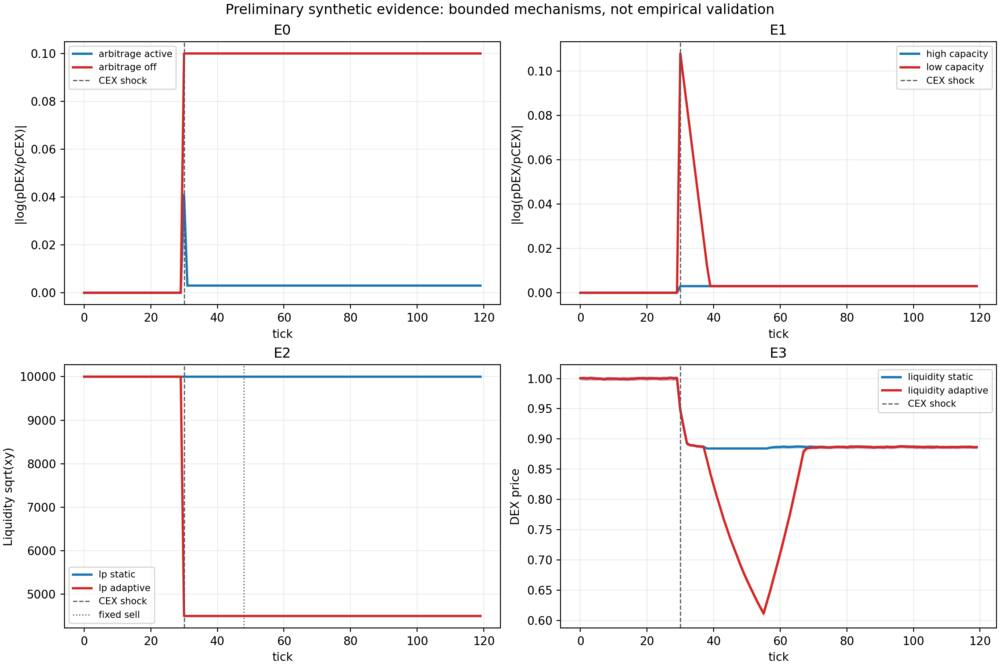
\includegraphics[width=\textwidth]{figures/preliminary-results.jpg}
\caption{Preliminary synthetic evidence. E0 and E1 show tracking error; E2 shows
liquidity withdrawal before a fixed sale; E3 shows transient amplification under the
adaptive LP rule. Bands represent the 25th--75th percentiles where seed variation is
present.}
\end{figure}

\section{Reproducible playground and technology transfer}

\subsection{Architecture}

A deterministic event engine will execute the AMM, arbitrage, policies, and
accounting. The pseudo-random generator will be fixed, with separate streams per
component; shocks and event ordering will be configurable and recorded. Each run
will produce a \texttt{run-id}, configuration file, commit SHA, environment version,
seeds, time series, metrics, invariant checks, and cryptographic checksums for its
artifacts.

\subsection{Canonical implementation reference}

The public, versioned architecture reference is the \textit{Master-s-thesis}
repository \cite{calderon2026repository}. In this version, the compilable manuscript
is published in \texttt{thesis/preprint}; the CPMM prototype and its analysis are
published in \texttt{experiments/cex\_dex\_preliminary}. These paths identify the
architecture and its versions; each run artifact also retains its own commit SHA,
configuration, and seed. No branch, URL, or synthetic result is interpreted as
empirical market evidence.

\subsection{Reproduction contracts}

\begin{enumerate}
  \item Versioned YAML configurations, specified economic units, and locked
    dependencies (\texttt{uv.lock} or equivalent).
  \item Swap, positive-reserve, inventory, and net-conservation checks, with explicit
    rules for fees and withdrawals.
  \item Stable commands: \texttt{run one}, \texttt{run sweep}, \texttt{analyze},
    \texttt{verify}, and \texttt{reproduce figure}. The current prototype is reproduced
    with \texttt{python3 experiments/cex\_dex\_preliminary/cex\_dex\_preliminary.py}
    and arguments \texttt{--output output/preliminary\_simulations --seeds 100}.
  \item CI with reference simulations and documented numerical tolerances; extensive
    results can live in artifact storage rather than Git.
  \item A synthetic dataset as the primary reference and a bounded empirical dataset
    with license, provenance, timestamps, and ingestion scripts.
\end{enumerate}

\subsection{Relationship to open market software}

The theoretical market will use CPMM mechanics compatible with a Uniswap v2-style AMM
\cite{adams2020uniswap,angeris2020cfmm}; it will not be extrapolated to concentrated
liquidity positions in Uniswap v3/v4 without testing. Swaps are proposed to be checked
against locally deployed reference contracts using Foundry/Anvil and Web3 libraries,
under controlled configuration and without real funds. For the CEX reference, public
series may be obtained through market adapters such as CCXT or a public exchange API,
after checking licenses, pair identity, latency, spreads, and timestamps. An optional
second level is replay of indexed on-chain events (for example, compatible pool Swap
and Sync records) to validate execution-error magnitudes. Running mainnet nodes,
advanced MEV, or live trading is not required.
